\chapter{RESULTS}

\graphicspath{ {./results/} }
%%%%%%%% This line gets rid of page number on first page of text
\thispagestyle{empty}

%%%%%%%%%%%%%

In this section, I provide qualitative research results and essential findings from prototype user testing spanning over multiple iterations over the course of thesis research and prototype development. 

\section{Visual Analysis}

The critical finding from the research highlights that the representations learned by the image recognition models are highly receptive to visualization, in large part because they are representations of visual concepts. I used image localization technique and gradient computation to visualize relevance heatmap, which substantiates image attribution and feature activation graph highlighting learned representations. For both methods, I use the VGG16 model, a convolutional neural network model trained on the ImageNet database.

\section*{Sensitivity Analysis}

% {images/colorful-group-of-birds.png}
% {images/heatmap-class-activations.png}

\begin{figure}
     \centering
     \begin{subfigure}[b]{0.45\textwidth}
         \centering
         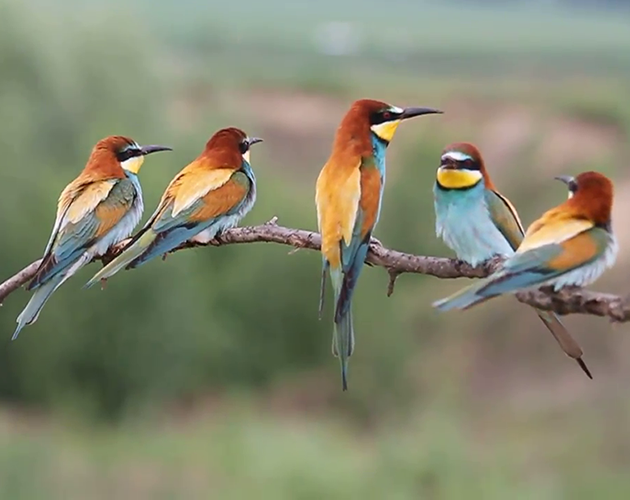
\includegraphics[width=\textwidth]{images/birds-2.png}
         \caption{Labeled Image}
         \label{fig:group-of-birds}
     \end{subfigure}
     \hfill
     \begin{subfigure}[b]{0.35\textwidth}
         \centering
         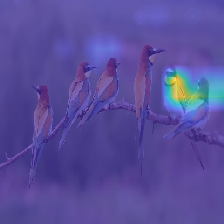
\includegraphics[width=\textwidth]{images/hm-layer-17.png}
         \caption{Relevance Heatmap}
         \label{fig:heatmap-birds}
     \end{subfigure}
        \caption{Sensitivity Analysis}
        \label{fig:sensitivity-analysis}
\end{figure}

DeepViz tool produces relevance heatmap as visual evidence to the class prediction that justifies the target class by highlighting the discriminating region corresponding to the desired class clearly. This method is useful to understand precisely which part of an image identified to belong to a specific class or category (class names known to VGG16), and thus allows localizing objects in images.

Figure 3.4 shows the sample explanation which first declares a predicted class label, which is correctly classified as "bee-eater", followed by relevance heatmap to elucidate why the model arrived at this decision. The relevance heatmap visualizes the importance of each pixel in the given image inconsistent with the predicted class. In this example, the bee-eater's beak and the neck are the basis for the model's decision. With the heatmap, the user can verify that the model works as intended.  This step validated the first premise of my hypothesis: Apply image localization and object detection technique to distinguish what part of an input image attributed most to the classification decision.
%The localized section of the image and intensity of filter activation are consistent in this case.

To examine instances where the incorrect label is predicted and identify what mistake a network is making, I collected a set of images that the VGG16 model fails to classify correctly. In this instance, when an example image is served to the tool seen in Figure 4.2. The model predicts the incorrect class. The input image is misclassified as "hare" when the correct label is a cat. The user can see why it predicted a wrong label by inspecting the heatmap visualization. Here, the model detected only the tail region and omitted other parts of the cat image, hence the feature extraction was not correct.

\begin{figure}
     \centering
     \begin{subfigure}[b]{0.39\textwidth}
         \centering
         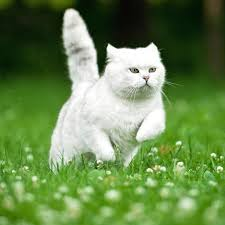
\includegraphics[width=\textwidth]{images/cat-hare-1.jpeg}
         \caption{Truth Label: Cat}
         \label{fig:cat}
     \end{subfigure}
     \hfill
     \begin{subfigure}[b]{0.39\textwidth}
         \centering
         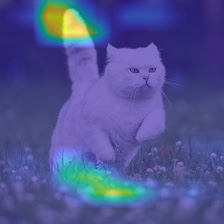
\includegraphics[width=\textwidth]{images/cat-hm-1.png}
         \caption{Predicted Class: Hare}
         \label{fig:hare}
     \end{subfigure}
        \caption{Misclassification Example}
        \label{fig:incorrect-prediction}
\end{figure}

To take this a step further, I breakdown the attention map at layer level to visualize the localization of the relevant image region at each hidden layer (Figure 4.3 and Figure 4.4). It helps carefully study the differential aspect of the attention map as it builds up towards the final layer. User can click through layer buttons to generate the heatmap corresponding to that hidden layer.

\begin{figure}
     \centering
     \caption{Layer-wise Relevance Heatmap}
     \vspace{1em}
     \begin{subfigure}[b]{0.30\textwidth}
         \centering
         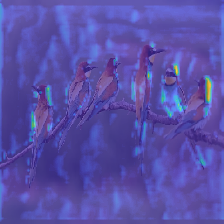
\includegraphics[width=\textwidth]{images/hm-layer-5.png}
         \caption{Layer 5 block2-conv2}
         \label{fig:layer-5}
     \end{subfigure}
     \hspace{1em}%
     \begin{subfigure}[b]{0.30\textwidth}
         \centering
         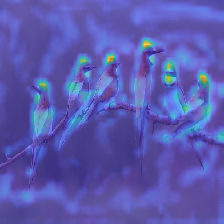
\includegraphics[width=\textwidth]{images/hm-layer-7.png}
         \caption{Layer 9 block3-conv3}
         \label{fig:layer-9}
     \end{subfigure}
     \hspace{1em}%
     \begin{subfigure}[b]{0.30\textwidth}
         \centering
         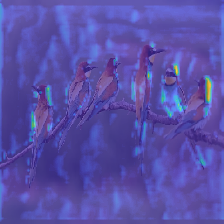
\includegraphics[width=\textwidth]{images/hm-layer-9.png}
         \caption{Layer 13 block4-conv3}
         \label{fig:layer-13}
     \end{subfigure}
     %\vspace{1em}%
     \begin{subfigure}[b]{0.30\textwidth}
         \centering
         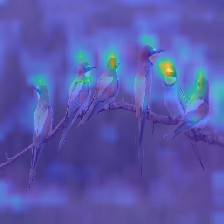
\includegraphics[width=\textwidth]{images/hm-layer-13.png}
         \caption{Layer 17 block5-conv3}
         \label{fig:layer-17}
     \end{subfigure}
    
    \label{fig:three graphs}
    
    \vspace{.5em}%
    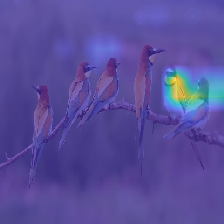
\includegraphics[width=0.35\textwidth]{images/hm-layer-17.png}
    \vspace{1em}%
    \caption{Final Layer Visualization}
    \label{fig:DeepViz - Visual Explanation Tool}

\end{figure}

\clearpage
\section*{Feature Activation Graph}

DeepViz visualizes activation output of the intermediate layers as a directed acyclic graph displaying how network builds up its internal representation. The graph decomposes feature activation map at each segment into a distribution of channels. The tool visualizes only selected channels considering the browser rendering and computation required.

This visualization helps the user understand how successive layers of the network transform the input image. Visualizing intermediate activations helps display the feature maps produced by various convolution and pooling layers in the network. User can see that nodes in the first layer mainly detects edges, where activations are retaining most of the information from the input image. As it moves deeper, the activations become highly abstract and far less visually interpretable. This is due to the network focusing on the higher level concepts like a dog's ear or bird's beak. These high-level activations carry less spatial information about the image and more class-specific information. This shows how the input image is continuously transformed at intermediate layers to distill out irrelevant information and retain useful information specific to the target class.

In summary, DeepViz visualization helped answer two important questions:
\vspace{-1em}
\begin{itemize}
\item  Why did the network think this image contained a bee-eater bird?
\vspace{-1em}
\item Where is the bee-eater located in the picture?
\end{itemize}
\vspace{-1em}
In particular, what is most exciting to note is that the head region of the fourth bird, which is the largest of all six birds are strongly activated: this is probably how the network can tell the difference between bee-eater and any other bird.

%\section{User Study}
\vspace{-1em}
\section{User Testing}

Having established that, next I evaluated whether the visualization can lead an end user to trust the model appropriately. Does it help user trust the model based on relevance heatmap as the visual evidence for the prediction made by the model? For this experiments, I conducted a human study where users tested several images using DeepViz tool to compare the heatmap visualization and predicted class for correct and incorrect classification.

\begin{figure}
     \centering
     \caption{User Testing Example of Correct and Incorrect Classification}
     \vspace{1em}
     \begin{subfigure}[b]{0.30\textwidth}
         \centering
         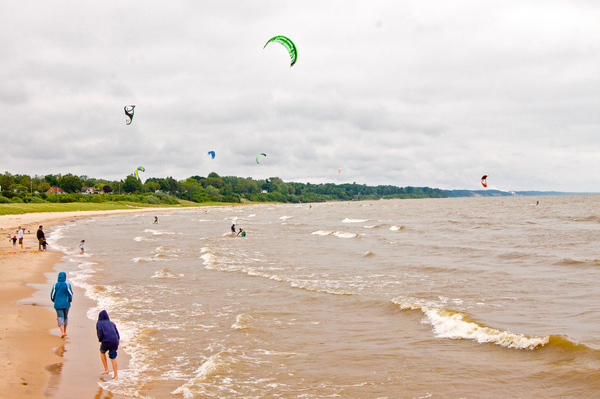
\includegraphics[width=\textwidth]{images/seashore.jpeg}
         \caption{True Label: Seashore}
         \label{fig:layer-5}
     \end{subfigure}
     \hspace{1em}%
     \begin{subfigure}[b]{0.30\textwidth}
         \centering
         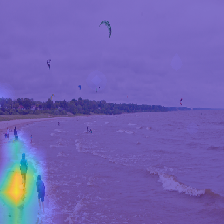
\includegraphics[width=\textwidth]{images/seashore-hm.png}
         \caption{Prediction: Seashore}
         \label{fig:layer-9}
     \end{subfigure}
     %vspace{0.5em}
     
     \vspace{0.5em}
     \begin{subfigure}[b]{0.30\textwidth}
         \centering
         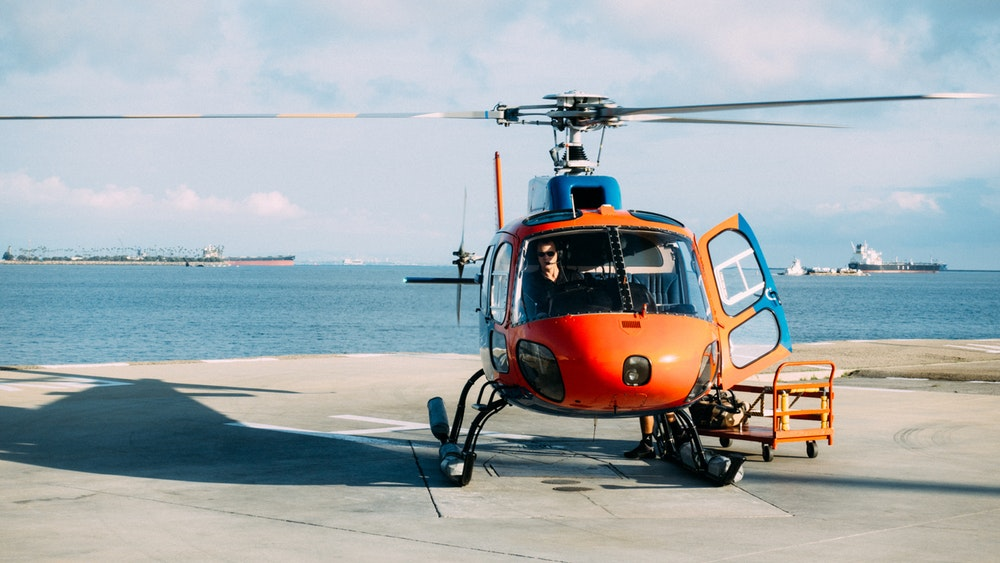
\includegraphics[width=\textwidth]{images/chopper-1.jpeg}
         \caption{True label: Helicopter}
         \label{fig:layer-5}
     \end{subfigure}
     \hspace{1em}%
     \begin{subfigure}[b]{0.30\textwidth}
         \centering
         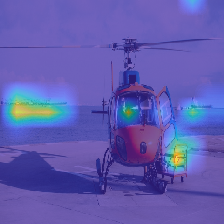
\includegraphics[width=\textwidth]{images/lifeboat-hm.png}
         \caption{Prediction: Lifeboat}
         \label{fig:layer-9}
     \end{subfigure}
     
     \vspace{0.5em}
     \begin{subfigure}[b]{0.30\textwidth}
         \centering
         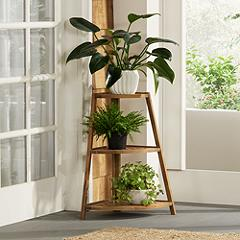
\includegraphics[width=\textwidth]{images/house-plant.jpeg}
         \caption{True label: Houseplant}
         \label{fig:layer-5}
     \end{subfigure}
     \hspace{1em}%
     \begin{subfigure}[b]{0.30\textwidth}
         \centering
         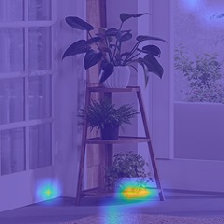
\includegraphics[width=\textwidth]{images/sliding-door-hm.png}
         \caption{Prediction: Sliding Door}
         \label{fig:layer-9}
     \end{subfigure}
     
     \vspace{0.5em}
     \begin{subfigure}[b]{0.30\textwidth}
         \centering
         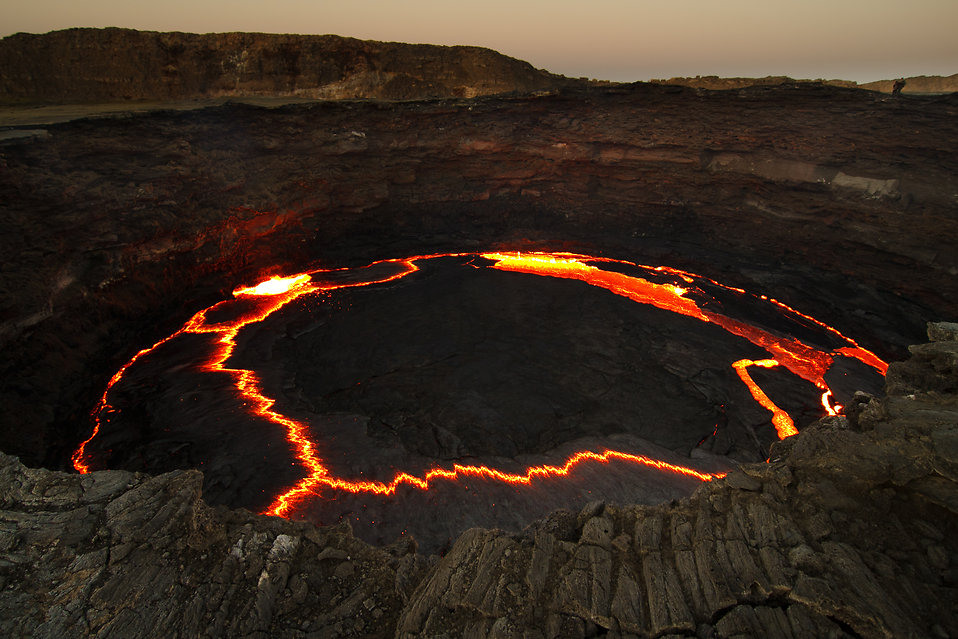
\includegraphics[width=\textwidth]{images/volcano-1.jpg}
         \caption{True label: Volcano}
         \label{fig:layer-5}
     \end{subfigure}
     \hspace{1em}%
     \begin{subfigure}[b]{0.30\textwidth}
         \centering
         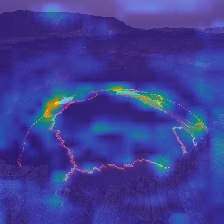
\includegraphics[width=\textwidth]{images/volcano-hm.png}
         \caption{Prediction: Volcano}
         \label{fig:layer-9}
     \end{subfigure}
\end{figure}


\iffalse % ----- START THE CUT ---------
%Given two prediction explanations, we want to evaluate; which seems more trustworthy
%Thus our visualization can help users place trust in a model that can generalize better, just based on individual prediction explanations.
%we select images from VOC 2007 val set that contain exactly two annotated categories and create visualizations for each one of them
%
%We compare generated explanations and definitions. All explanations on the left include an attribute which is not present on the image on the right. In contrast to definitions, our explanation model can adjust its output based on visual evidence. (Color figure online) 
%Incorrect Prediction. We qualitatively examine explanations for instances where the incorrect label is predicted (Fig. 8). In these scenarios, explanations are frequently image relevant and mention features common in both the image instance and the predicted class. For example, in the first row of Fig. 8 the model mistakes the “Laysan Albatross” for the “Cactus Wren”. The explanation text
%includes many features also mentioned in the “Cactus Wren” definition (for example color and the spotted feathers) and is relevant to the image.
%We compare generated explanations and definitions. All explanations on the left include an attribute which is not present on the image on the right. In contrast to definitions, our explanation model can adjust its output based on visual evidence.
\fi % ---------- END THE CUT -----------
